\documentclass[onecolumn, draftclsnofoot,10pt, compsoc]{IEEEtran}
\usepackage{graphicx}
\usepackage{url}
\usepackage{setspace}
\usepackage{cite}
\usepackage{geometry}
\usepackage{enumitem}


\geometry{textheight=9.5in, textwidth=7in}

% 1. Fill in these details
\def \CapstoneTeamName{Audio Extravaganza}
\def \CapstoneTeamNumber{26}
\def \GroupMemberOne{Martin Barker}
\def \GroupMemberTwo{Devon Cash}
\def \GroupMemberThree{Alexander Niebur}
\def \GroupMemberFour{Mason Sidebottom}
\def \GroupMemberFive{Ben Windheim}
\def \CapstoneProjectName{Audio Extravaganza}
\def \CapstoneSponsorCompany{Oregon State University}
\def \CapstoneSponsorPerson{Kristen Winters}

% 2. Uncomment the appropriate line below so that the document type works
\def \DocType{		
                %Problem Statement
				Requirements Document
				%Technology Review
				%Design Document
				%Progress Report
				}
			
\newcommand{\NameSigPair}[1]{\par
\makebox[2.75in][r]{#1} \hfil 	\makebox[3.25in]{\makebox[2.25in]{\hrulefill} \hfill		\makebox[.75in]{\hrulefill}}
\par\vspace{-12pt} \textit{\tiny\noindent
\makebox[2.75in]{} \hfil		\makebox[3.25in]{\makebox[2.25in][r]{Signature} \hfill	\makebox[.75in][r]{Date}}}}
% 3. If the document is not to be signed, uncomment the RENEWcommand below
\renewcommand{\NameSigPair}[1]{#1}

%%%%%%%%%%%%%%%%%%%%%%%%%%%%%%%%%%%%%%%
\begin{document}
\begin{titlepage}
    \pagenumbering{gobble}
    \begin{singlespace}
        \hfill  
        \par\vspace{.2in}
        \centering
        \scshape{
            \huge CS Capstone \DocType \par
            {\large\today}\par
            \vspace{.5in}
            \textbf{\Huge\CapstoneProjectName}\par
            \vfill
            {\large Prepared for}\par
            \Huge \CapstoneSponsorCompany\par
            \vspace{5pt}
            {\Large\NameSigPair{\CapstoneSponsorPerson}\par}
            {\large Prepared by }\par
            Group\CapstoneTeamNumber\par
            % 5. comment out the line below this one if you do not wish to name your team
            \CapstoneTeamName\par 
            \vspace{5pt}
            {\Large
                \NameSigPair{\GroupMemberOne}\par
                \NameSigPair{\GroupMemberTwo}\par
                \NameSigPair{\GroupMemberThree}\par
                \NameSigPair{\GroupMemberFour}\par
                \NameSigPair{\GroupMemberFive}\par
            }
            \vspace{20pt}
        }
%         \begin{abstract}
%         %UNCOMMENT WHEN OTHER CITATIONS ARE ADDED
%         % \cite{ph}
%         % 6. Fill in your abstract    

		
% 		\end{abstract}     
    \end{singlespace}
\end{titlepage}
\newpage
\pagenumbering{arabic}
\tableofcontents
% 7. uncomment this (if applicable). Consider adding a page break.
%\listoffigures
%\listoftables

% Uncomment to make table of contents full page
\clearpage

% 8. now you write!


\clearpage

\section{Introduction}
% Martin
\subsection{Purpose}
For our effects pedal, we will be developing a system to meet the needs of musicians and musical artists. Our product will need to operate in live musical performance environments, as well as in recording situations. Due to these requirements, it will be essential that out effects pedal can be operated easily and consistently with no technical hiccups, crashes, or unexpected results. Mitigating latency will also be crucial for developing a pedal capable of holding up in a recording environment, as well as ensuring that our system produces high quality audio with no hiss or buzz. 
Our stakeholders will primarily be people with a connection to music. Although music will be a shared trait, our users are expected to vary in terms of technical capabilities and experience using audio effects pedals. A common expectation for these users will be that our pedal is easy to operate, regardless of how experienced somebody is with effects pedals.\\
Our product's requirements will have to fit our stakeholders needs, in that we are able to create an easy-to-use yet powerful effects pedal capable of producing reliable audio that a performer can actually use during a concert. 

% Martin 
\subsection{Scope}
    \begin{enumerate}[label=\alph*.]
        \item Software product(s) to be produced by name: pedalProject - Final name to be determined at a later date.
        \item What it does: This effects pedal will improve the lives of musicians by providing an easy to use and reliable effects pedal which can hold up during live performances.
        \item Benefits/objectives/goals: Our pedal will provide benefits to the musician by giving them the ability to recursively apply effects to a looping sample, which can be changed to only affect certain previous or future loops. Our objectives are to extensively plan out our design, implement it in software, and to then move it to hardware. Our goals are to create the software for our system so that it is easily modifiable by the user, and allows for future modifications/additions into our pedal.
\end{enumerate}

\subsection{Product Overview}
    \subsubsection{Product Perspective}
    Our product will take influence from other currently available looping pedals, and will build on their designs to create something more user friendly and easily modifiable. 
    Seeing as effects pedals are often a part of larger effects chains, we will need to include audio input and output ports on our looping pedal, which our software will be able to interpret and output. 
    
    \subsubsection{Product Functions}
    Our product functions are as follows:
    \begin{enumerate}[label=\alph*.]
        \item Looping effect allowing the user to apply other effects to looping samples.
        \item The modulation of incoming audio through the application of audio effects.
        \item The addition for more effects to be added by the user easily.
    \end{enumerate}
    
    \subsubsection{User Characteristics}
    Our system will have users who are musicians with experience using multiple effects pedals, musicians with no experience using effects pedals, and non-musicians with a primary focus on the two preceding groups. The user will also act as a maintainer of the system, with the ability to apply more effects to the system based on our documentation. 
    
    \subsubsection{Limitations}
    There will be some hardware limitations, such as how much information we are able to store on a small single-board computer, as well as what audio quality we are able to achieve with and without using an external sound card. Reliability will be a limitation in that we need to focus on achieving a certain level of reliability above everything else. If our pedal has amazing sounding effects but the looping feature has unreliable latency or cuts out, it will not meet our standards for this project. 
    
% \subsection{Definitions}




% \bibliographystyle{IEEEtran}
% \bibliography{./refs.bib}

\section{Specific Requirements}

\subsection{External Interfaces}
% martin
One stretch goal of our project is to implement an external mobile interface which the user can use to communicate with the effects pedal. This interface would either be a mobile application or website which would connect to the user's pedal over USB (\ref{USB}), Bluetooth, or WiFi connection. The external interface would allow the user to edit and save presets for the available effects supported by the pedal, which could then be transferred to the pedal. These presets would store information on a certain effect, such as options for looping control of time / delay / chaining of other effects. 

\subsection{Functions}
% Mason and Martin
        % Add plug and play
    \subsubsection{Base System}
    \begin{enumerate}[label=\alph*.]
        \item The system shall convert all incoming audio signals to a digital signal via DAC (\ref{DAC}). % This may fall under hardware
        \item The system shall convert all outgoing audio signals to an analog signal via DAC (\ref{DAC}).
        \item The system shall map a function to each hardware interface.
        \item The system shall display pertinent information via an LCD (\ref{LCD}) screen.
        \item The system shall start all subsystems on power up.

    \end{enumerate}
    
    \subsubsection{Looping Sub System}
        \begin{enumerate}[label=\alph*.]
            \item The system shall allow users to start and stop recording input via a pedal.
            \item The system shall allow users to start and stop playback via a pedal interface.
            \item The system shall allow users to toggle recording or playback via a pedal.
            %Can change # here


        \end{enumerate}
    
    \subsubsection{Modulation Sub System}
    \begin{enumerate}[label=\alph*.]
        \item The system shall allow users to select effects to toggle for each pedal.
        \item The system shall allow users to load effect presets.
        \item The system shall allow users to modify effect parameters.
    \end{enumerate}
    
    \subsubsection{Stretch Functionality}
    \begin{enumerate}[label=\alph*.]
        \item The user shall be able to create their own effects and patches on an external device.
        \item The user shall be able to upload their effects and patches from an external device.
        \item The user shall be able to download saved looper recordings as files to an external device.
        \item The user shall be able to upload recordings from an external device.
        \item The system shall allow input from external devices, like a MIDI (\ref{MIDI}) controller, via USB.
        \item The system shall cache up to 4 recordings, for toggling with pedals.
     \item The system shall allow users to save recording presets for retrieval later.
            %   Maybe
     \item The system shall allow users to select an interval in beats per minute to quantize recordings.
            % Similar to a launch pad behavior
    \item The system shall allow users the queue output to play on the next measured interval.
            \item The system shall allow users to save modifications as a preset.
    \end{enumerate}

\subsection{Usability Requirements}
% Alex and Devon
% Measurable effectiveness, efficiency, and satisfaction requirements
    \begin{enumerate}[label=\alph*.]
        \item The system should require no additional configuration on boot, and be ready to function within 2.5 seconds. % Give us a bit of a buffer around our ideal 1 second boot
        \item The hardware enclosure should be designed in a way to not destroy the system when kicked, dropped, or stored. % Able to survive wear and tear (perhaps 25 pounds of force?)
        \item All hardware and software controls should be labelled with the name and state of the variable they modify.
        \item Any selection hierarchies in the control system should be three levels or less.
        \item Users should be able to locate and select known effects within 10 seconds. % Generous time constraint -- we can restrict it later if need be
        \item Users should be able to create and deploy a scene of already selected effects within 10 seconds.
        \item Users should be able to interact with the looping system without modifying currently applied effects.
        \item All hardware and software controls should have perceivable effects within 250 ms of giving it an input.
        % User opinion/perception
        \item Minimum 80\% of users should report a pleasant user experience.
        % Memorability
        \item Minimum 80\% of users should display evidence of retaining aptitude between test sessions.
        % Learnability
        \item Inexperienced users should show a minimum 20\% increase in speed each time a task is repeated.
        
    \end{enumerate}

\subsection{Performance Requirements}
% Ben and Devon
% Here are a couple metrics to think about - Devon
Some requirements that can be attached to the performance aspect of our product are vital, due to the very performance nature of our project. Regarding the looping aspect of our product, we must limit the latency (input-to-output) delay to a unnoticeable level, and uniformly for bypassed, engaged, and high-processing modes. While we do not have a reasonable estimate for the amount of loop layers to include, we are ambitious and wish for that to be a simple scale to increase upon. \\
In regards to the effects, we can require two concurrent effects to run without any incurred latency, and we can require a deterministic effect configuration, such that the same input parameters produce the same output parameters (this does account for the variance in input signal from different kinds of sources). \\
Another realm of requirement is in the mobility and encasing of our product. The mobility and stability should be comparable to similar effects, and the setup time should be similar as well, such that a user is not prohibited by their ability to quickly move, use, and apply pressure to the product. \\
In the event that we can implement an external interface, it should follow similar requirement guidelines to the rest of the product. There should be little latency, and file transfer and upload should be achieved at a high rate. 
%Looper:
 %   delay compensation
  %  Less than x ms of delay
   % up to x number of overdubs?
% Effects:
%     Apply x number of effects concurrently without delay
%     Bypass delay limit?
%     Maintain and apply x configurations
%     Finish with x number of effects
% Pedal Enclosure:
%     Withstand x amount of force
%     Fit within a pre-determined volume
% Stretch: External Interface:
%     Allow file transfer at a high(?) rate
%     Ms delay for live control?
    
    

\subsection{Design Constraints}
% Ben and Mason
% Specify constraints on the system design imposed by external standards, regulatory requirements, or project limitations
    \begin{enumerate}[label=\alph*.]
        \item The monetary cost of the final product should be under \$300 USD to maintain its viability as a cheaper alternative.
        \item The hardware input will be constrained by the number of GPIO (\ref{GPIO}) pins available on the board. Digital Audio Converter, and LCD display will use a fair amount for output.
        \item The number of concurrent effects will be constrained by the processing power of the single-board computer that is used.
        \item The size of the product will be constrained to portability standards.
        \item The ports for external input -- audio signals, MIDI (\ref{MIDI}) signals, etc. -- will be constrained by industry standards for input.
    \end{enumerate}

\subsection{Software System Attributes}
% Alex and Devon
% Performance metrics section of problem statement
    \begin{enumerate}[label=\alph*.]
        \item The final product should be able to perform without any errors when in use.
        \item Interfacing with our product should be easy to understand for both people new to the product, and those who are experienced in the field.
        \item The MSRP (\ref{MSRP}) of the final product should be affordable for people new to the world of music technology.
        \item The final product will need a lightweight operating system in order to allow for quick startup, and maximize hardware performance.
    \end{enumerate}

%\subsection{Supporting Information}
%There are several options available for us for a variety of different aspects for this project.
%The following scenarios are not requirements for what we will use in our final product, but instead serve as a reference in our options on receive and send audio signals while processing them.
    %\begin{enumerate}[label=\alph*.]
        %\item For our input/output connectors, we have options that are common in the professional sphere, such as the 1/4 inch cable, XLR cable, or an input that supports both of these input/output connections.
        %\item Our single-board computer can also vary from a general purpose system such as a Raspberry Pi or Arduino to an easily modifiable, but less user friendly, FPGA (\ref{FPGA}).
    %\end{enumerate}
% Re-evaluate after most of document is done as a team

\newpage
Gantt Chart\\
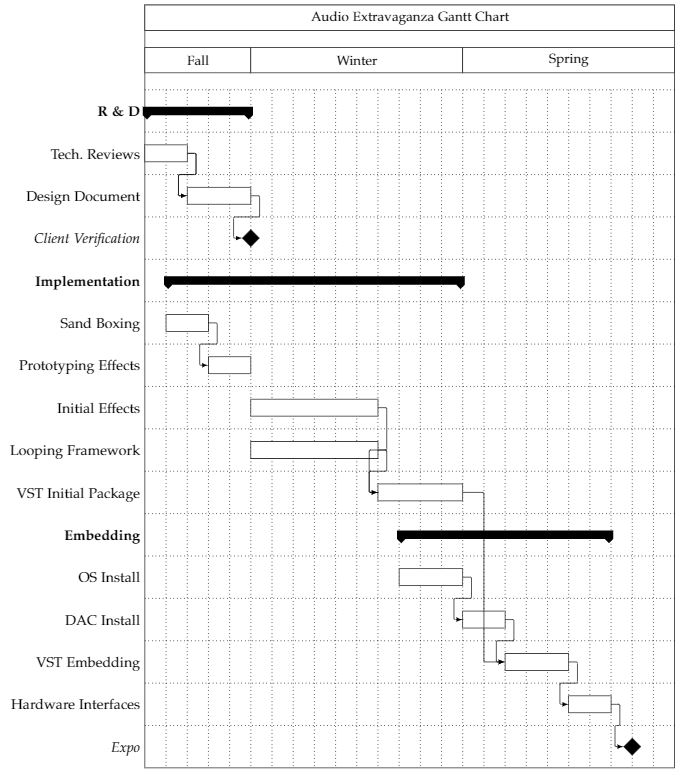
\includegraphics[width=0.8\textwidth]{./gantt.JPG}
%
%5 weeks in fall left, 10 per other terms

\begin{ganttchart}[vgrid, hgrid]{1}{25}
        \gantttitle{Audio Extravaganza Gantt Chart}{25} \\
        \gantttitle{Fall}{5}            
        \gantttitle{Winter}{10}
        \gantttitle{Spring}{10} \\
        
        \ganttgroup{R \& D}{1}{5} \\
            \ganttbar[name=r1]{Tech. Reviews}{1}{2} \\
            \ganttbar[name=r2]{Design Document}{3}{5} \ganttnewline
            \ganttmilestone[name=r3]{Client Verification}{5} \ganttnewline
        \ganttgroup{Implementation}{2}{15} \\
            \ganttbar[name=i1]{Sand Boxing}{2}{3} \\
            \ganttbar[name=i2]{Prototyping Effects}{4}{5} \ganttnewline
            \ganttbar[name=i3]{Initial Effects}{6}{11} \ganttnewline
            \ganttbar[name=i4]{Looping Framework}{6}{11} \ganttnewline
            \ganttbar[name=i5]{VST Initial Package}{12}{15} \ganttnewline
        \ganttgroup{Embedding}{13}{22} \\
            \ganttbar[name=e1]{OS Install}{13}{15} \\
            \ganttbar[name=e2]{DAC Install}{16}{17} \ganttnewline
            \ganttbar[name=e3]{VST Embedding}{18}{20} \ganttnewline
            \ganttbar[name=e4]{Hardware Interfaces}{21}{22}\ganttnewline
        
        \ganttmilestone[name=expo]{Expo}{23}
        
        \ganttlink{r1}{r2}
        \ganttlink{r2}{r3}
        \ganttlink{i1}{i2}

        \ganttlink{i3}{i5}
        \ganttlink{i4}{i5}
        \ganttlink{i5}{e3}
        \ganttlink{e1}{e2}
        \ganttlink{e3}{e4}
        \ganttlink{e2}{e3}
        \ganttlink{r1}{r2}
        \ganttlink{e4}{expo}
    \end{ganttchart}

\newpage
\section{Verification}

%\subsection{External Interfaces}

\subsection{Functions}
% Mason & Martin
% we already wrote this in the requirements.tex file?
    
    To verify the functionality of our product, we will run rigorous unit tests on each proposed function. While combining functionality, we will run integration tests to make sure that the overall product performs as expected with the subsystems connected. After combining any two functions, we will also need to run regression tests to make sure that the new modifications or additions did not impact the performance or output of any other component of the system.
    
   
\subsection{Usability Requirements}
% Alex & Devon
The usability standards established in Section 2.3 which provide concrete values (input response times, labelling standards, etc.) can be evaluated using appropriate measurement methods, or by simple observation of the product. Impression and opinion based user requirements will be collected from testing groups through standardized scales (1 - 10 rating). Requirements reliant on user actions will be measured based on observed usability sessions conducted with qualified individuals. User tests will be conducted with a diverse set of potential users including multiple levels of skill with electronic systems (musical and non-musical) and music. 

%Once our product is plugged into a power system, it should take at maximum one second for it to start generating the effects. This will be done using system outputs and testing\\
%Our testing of clearly defined features will be based off user feedback from our testing groups using a one to ten rating scale.\\
%The time to select an effect, trigger loop functionality, and create new scene configurations will be determined by timing 

\subsection{Performance Requirements}
From a performance standpoint, we can verify that the final product is operating per the specifications by performing a series of measurements and qualitative assessments. For measurable data, we can look assure the latency (the delay from input to output) is unnoticeable and is not additive in each subsequent loop. This likely means limiting acceptable latency to approximately 10ms. We can also approach this latency metric from the amount of processing we are doing for a signal. Latency should be very uniform regardless of the level of effects processing we are incurring, and should also be comparable to when the effects are engaged or in bypass mode. We can also verify that the device is maintaining its configurations and that the same effects are deterministic of the parameters. Finally, within the limitations of quantification, we can verify that the portability of the product will be comparable to other similar products, and that the mobility and implementation of the product is not an inhibitory factor to a performer. \\
Shifting to a more qualitative point of view, we can verify that the performance capabilities are on par by gaining feedback from performers on all levels of skill and experience. Perhaps the best way to determine if we have some performance-worthy product is by conducting surveys with the users themselves. We can also similarly ask audiences for their impressions, and we can try to gain valuable information from that to verify if the product performs as expected. 


\subsection{Design Constraints}
% Ben & Mason
The design constraints are fairly straightforward, factoring in cost and physical limitations of the equipment we are trying to use. To verify our product against the design constraints, we can check to make sure our goals were met while making sure we stay within the constraints of our project. One of these main constraints is the overall cost-to-make and potential price-to-purchase. While we wish our product to be robust, powerful, and unique, it cannot be prohibitively expensive, and there may be some areas of contention and trade-off between versatility and power over economics and simplicity. Additionally, we are at the mercy of hardware and software limitations, and while our research suggests all goals and stretch goals are possible, it is important to be able to deal with compromising in some areas. To verify our product fits within the design constraints, we must compare our costs and our goals to our final implementation and assure that our constraints were followed as closely as possible. 

\subsection{Software System Attributes}
% Alex
Verifying the reliability and ease of learning will be judged by our testing groups, using a one to ten rating scale. Our cost aspect will be monitored by the costs that go into making our final product. Lastly, testing the system boot time will either require using computer output, either to a monitor with the boot time or lighting up an onboard LED if we boot before a set time, or using external hardware such as video/audio to determine the time between plug-in and fully being on.

%\subsection{Supporting Information}


\section{Appendices}

\subsection{Assumptions and Dependencies}
    %add \label{some name}
    % use \ref{labelname} in text to refer to here
\subsection{Acronyms and Abbreviations}
    \begin{itemize}
        \item \label{DAC} \textbf{DAC:} Digital Audio Converter.
        %\item \label{FPGA} \textbf{FPGA: } Field-Programmable Gate Array
        \item \label{GPIO} \textbf{GPIO:} General Purpose Input/Output
        \item \label{LCD} \textbf{LCD:} Liquid-Crystal Display.
        \item \label{LED} \textbf{LED:} Light-Emitting Diode.
        \item \label{MIDI} \textbf{MIDI:} Musical Instrument Digital Interface.
        \item \label{MSRP} \textbf{MSRP:} Manufacturer's Suggested Retail Price.
        \item \label{USB} \textbf{USB:} Universal Serial Bus
        \item \label{DAM} \textbf{DAM:} Digital Audio Manipulation
    \end{itemize}

\end{document}
